\section{Sziták}
\label{sec:szitak}

A \texttt{gui} program tartalmazza Eratoszthenész szitájának több megvalósítását.
Ezek az implementációk mind szegmentáltak, azaz csak egy rövidebb intervallumon szitálnak,
és annak befejezéséig nem kezdenek bele új intervallumba.
Egy intervallum szitáláshoz szükséges az intervallum végének négyzetgyökéig a prímek listája.
A prímeket ismerve maradékos osztással meghatározható, hogy melyik a legkisebb többszörösük, ami legalább akkora, mint az intervallum kezdete, és onnantól összeadással az intervallum végéig meghatározható a többi többszörösük.
A \ref{alg:eratosthenes-segment} algoritmus ezt írja le.

\begin{algorithm}
\floatname{algorithm}{Algoritmus}
\caption{Az $[u, v[$ intervallum szitálása}
\label{alg:eratosthenes-segment}
\begin{algorithmic}[1]
\State legyenek a számok az $[u, v[$ intervallumban megjelöletlenek
\For{$p \in \{\textrm{prímek}\sqrt{v-1}\textrm{-ig}\}$}
	\For{$f \gets p \left \lceil{\frac{u}{p}}\right \rceil ; v > f; f \gets f+p$}
		\State legyen $f$ megjelölve
	\EndFor
\EndFor
\For{$f \in [u, v[$}
	\If{$f$ nincs megjelölve}
		\State $f$ prím
	\EndIf
\EndFor
\end{algorithmic}
\end{algorithm}

Ha több egymás utáni intervallumot kell szitálni, akkor minden prímhez eltárolható, hogy melyik pozícióban fog legközelebb szitálni.
Ezzel az osztások időbeli költsége tárhely költségre váltható.
A legegyszerűbb megoldás a prím-pozíció párok tárolása egy tömbben.
A \ref{alg:eratosthenes-segments} algoritmus az $[u, v[$ intervallum szitálását írja le, ahol $v=u+kd$. Az algoritmus $k$ darab $d$ hosszú részintervallumot szitál.

\begin{algorithm}
\floatname{algorithm}{Algoritmus}
\caption{Az $[u, v[$ intervallum szitálása, $v=u+kd$}
\label{alg:eratosthenes-segments}
\begin{algorithmic}[1]
\State legyen $t$ egy tömb
\State $s \gets 0$ \Comment{a tömb elemeinek száma}
\For{$p \in \{\textrm{prímek}\sqrt{v-1}\textrm{-ig}\}$}
	\State $t[s] \gets (p: p, f: p \left \lceil{\frac{u}{p}}\right \rceil)$
	\State $s \gets s+1$
\EndFor
\For{$\ell \gets 1, v \gets u+d; k \ge \ell; \ell \gets \ell+1, u \gets u+d, v \gets v+d$}
	\State legyenek a számok az $[u, v[$ intervallumban megjelöletlenek
	\For{$i \in [1, s]$}
		\For{$; v > t[i].f; t[i].f \gets t[i].f+t[i].p$}
			\State legyen $t[i].f$ megjelölve
		\EndFor
	\EndFor
	\For{$f \in [u, v[$}
		\If{$f$ nincs megjelölve}
			\State $f$ prím
		\EndIf
	\EndFor
\EndFor
\end{algorithmic}
\end{algorithm}

A \texttt{gui} programban ''Eratoszthenész szitája'' ezt az algoritmust valósítja meg.
Ezzel a módszerrel a program minden rövid szegmensben a tömb minden elemét sorra veszi, azokat is, amik a szegmensben nem szitálnak.
A többi implementált eratoszthenészi szita összetettebb struktúrákkal próbálja kiválasztani a ténylegesen szitáló elemeket.
A többi implementált szita prioritásos sort használ az elemek részleges rendezéséhez, és sor elejének feldolgozásával választja ki a szegmensben szitáló elemeket.
A bináris kupac és az edénysort használó szita mellett a Cache Optimalizált Lineáris Szita is soron alapul.

\subsection{Prioritásos sorok}

A prioritásos soron alapuló szita algoritmusa nagyon hasonló a \ref{alg:eratosthenes-segments} algoritmushoz.
Az elemek sorban feldolgozása helyett a sor elejét addig veszi ki, amíg az az éppen szitált szegmensbe esik.
Ezekkel az elemekkel a szitálást elvégzi a szegmensben, majd a sorba visszahelyezi, már az új, mostani szegmensnél nagyobb pozícióval.
Az elemek sorrendjét a legközelebbi szitált pozíció határozza meg, a sor eleje az éppen szitált szegmenshez legközelebbi elem.
Az elemek sorrendjénél a szegmenseken belüli sorrend vizsgálata felesleges.
A prioritásos soron alapuló szitálás algoritmusát a \ref{alg:eratosthenes-queue} adja meg, a sor adatszerkezet meghatározása nélkül.
A tényleges megvalósítás az eltávolít-hozzáad sorműveletpár helyett a helyben módosítást és a struktúra invariánsának visszaállítását is választhatja.

\begin{algorithm}
\floatname{algorithm}{Algoritmus}
\caption{Az $[u, v=u+kd[$ intervallum szitálása, prioritásos sorral}
\label{alg:eratosthenes-queue}
\begin{algorithmic}[1]
\State legyen $q$ egy üres sor
\For{$p \in \{\textrm{prímek}\sqrt{v-1}\textrm{-ig}\}$}
	\State hozzáad$(q, (p: p, f: p \left \lceil{\frac{u}{p}}\right \rceil))$
\EndFor
\For{$\ell \gets 1, v \gets u+d; k \ge \ell; \ell \gets \ell+1, u \gets u+d, v \gets v+d$}
	\State legyenek a számok az $[u, v[$ intervallumban megjelöletlenek
	\While{$v > \min(q).f$}
		\State $(p, f) \gets \textrm{eltávolít-min}(q)$
		\For{$; v > f; f \gets f+p$}
			\State legyen $f$ megjelölve
		\EndFor
		\State hozzáad$(q, (p, f))$
	\EndWhile
	\For{$f \in [u, v[$}
		\If{$f$ nincs megjelölve}
			\State $f$ prím
		\EndIf
	\EndFor
\EndFor
\end{algorithmic}
\end{algorithm}

A \texttt{gui} program szitái közül ezt az algoritmust követi az edénysor szita, a bináris kupac szita, és a COLS körkörös listája is. A bináris kupac szitánál az eltávolítás-hozzáadás és a helyben javítás között a felhasználó választhat.

\subsection{Edénysor}

A edénysor egy monoton prioritásos sor.
Minden állapotához tartozik egy érték, a sor aktuális pozíciója, aminél kisebb vagy egyenlő pozíciójú értéket a sor nem tartalmazhat.
A sor pozíciójának megnövelése a sor elejének eltávolításával is együtt jár.
A sor edények egy végtelen sorozatát is tárolja, a sor elemei ezekbe az edényekbe kerülnek.
Egy eltárolt elem helyét az edények között az elem pozíciójának és a sor aktuális pozíciójának távolsága határozza meg.
Két szám távolságát egy számrendszerben két érték határozza meg, a legnagyobb helyiérték, amiben eltérnek a számjegyeik, és a nagyobbik szám számjegye ezen a helyiértéken.

Legyen $a \in \mathbb{N}, a > 1$ a sor számrendszerének alapszáma.
$x$ $i$-edik számjegyét $a$ alapú számrendszerben jelölje $x_i$, ahol $x \in \mathbb{N}_0$.
Legyen $h(x, y)$ a legnagyobb helyiérték, ahol $x$ és $y$ eltér.
A sor által használt $d(x, y)$ távolságfüggvény az $y-x$ eltérés nagyságrendjének közelítése.
\begin{equation}
x = \sum_{i=0}^{\infty} x_i a^i\ (i \in \mathbb{N}_0, x_i \in \mathbb{N}_0, x_i < a)
\end{equation}
\begin{equation}
h(x, y) = \max{\{i \in \mathbb{N}_0 | x_i \not= y_i\}}\ (x, y \in \mathbb{N}_0, x<y)\\
\end{equation}
\begin{equation}
\label{ddef}
d(x, y) = (a-1) h(x, y) + y_{h(x, y)} - 1
\end{equation}
Kettes számrendszerben a távolság logaritmussal és a bitenkénti kizáró-vagy művelettel is megadható,
\begin{align*}
d(x, y) = \lfloor log_2{(x \oplus y)} \rfloor
\end{align*}

Legyen $q$ egy edénysor
\begin{itemize}
\item $a$ alapszámmal
\item $p(q) \in \mathbb{N}_0$ a $q$ sor pozíciója
\item $b(q, i)$ a $q$ sor $i$. edénye\ $(i \in \mathbb{N}_0)$
\item $p(r) \in \mathbb{N}$ a $q$ sor egy lehetséges $r$ elemének pozíciója.
\end{itemize}
Ekkor a $q$ sor invariánsa:
\begin{align*}
\forall r \in q &: &\\ 
	& p(q) < p(r) \\
	& \forall i \in \mathbb{N}_0: r \in b(q, i) \iff i=d(p(q), p(r)) \\
\forall r \not\in q &: \forall i \in \mathbb{N}_0: r \not\in b(q, i)
\end{align*}
%%% P: lehet, hogy p(...) helyett f(...) kéne, ha már az algoritmusokban is az volt, ahol a p foglalt volt a prímekre.

Új sor létrehozásához az edények listáját kell létrehozni, a sor kezdő pozíciója bármi lehet.
Új elemet a sorhoz a távolságfüggvény kiértékelése után az elem edénybe szúrásával lehet adni,
az új $r$ elem az $b(q, d(p(q), p(r)))$ edénybe kell kerüljön.
Ez a művelet az invariánst fenntartja.

A sor pozíciójának eggyel megnövelésével a sor invariánsa kétféleképpen válhat hamissá:
\begin{itemize}
\item egy elem pozíciója és a sor pozíciója egyenlő lesz. A pozíció növelése művelet ezeket az elemeket a sorból eltávolítja, és a művelet eredményeként visszaadja.
\item az elem és a sor pozíciójának távolsága csökken. Az invariáns visszaállításához a művelet ezeket az elemeket áthelyezi az új távolság szerinti edénybe.
\end{itemize}
A sor elejének eltávolítsa az edénysornál tetszőleges számú elemet távolíthat el a sorból, és nem üres sor esetén is előfordulhat, hogy a sor elejének eltávolítása nem ad vissza elemeket.

\begin{algorithm}[H]
\floatname{algorithm}{Algoritmus}
\caption{A $q$ edénysor elejének eltávolítása}
\label{alg:buckets-remove-min}
\begin{algorithmic}[1]
\Function{eltávolít-min}{$q$}
	\State $l \gets$ üres lista
	\State $i \gets d(p(q), p(q)+1)$
	\State $p(q) \gets p(q)+1$
	\While{$b(q, i)$ nem üres}
		\State $r \gets$ eltávolít$(b(q, i))$
		\If{$p(r) = p(q)$}
			\State hozzáad$(l, r)$
		\Else
			\State hozzáad$(b(q, d(p(q), p(r)))$
		\EndIf
	\EndWhile
	\State \Return l
\EndFunction
\end{algorithmic}
\end{algorithm}

Az edénysor elejét ezzel az adatstruktúrával nem lehet hatékonyan lekérni az elemek eltávolítása nélkül.

Edénysorral szitáláskor a sor pozícióját a szegmens végéig növelve pontosan a szegmensben szitáló elemek kerülnek ki a sorból, a sor elejének lekérdezésére nincs szükség.
Ha a szegmensek hossza egy szám, akkor a prímek azok a számok, amelyik sorpozíciókra lépve a pozíció növelése nem távolít el elemet.

\subsubsection{Funkcionális megvalósítás}

Az edénysoron alapuló szitára tisztán funkcionális megoldás adható.
Az edénysor műveleteit láncolt listákkal számjegyenként ábrázolt számok összeadására lehet visszavezetni.
Az $x+y$ összeadás elvégzésével a $h(x, x+y)$ és a $d(x, x+y)$ is kiszámítható, $h(x, x+y)$ a helyiérték, ahol összeadás közben a kisebbik szám számjegyei és az átvitel is elfogy. A $d(x, x+y)$ meghatározásához az eredményből még a $h(x, x+y)$ helyiértéken lévő számjegyet is ki kell olvasni.
A számok láncolt listával ábrázolásával az $x+y$ kiszámítása $\theta(h(x, x+y))$ műveletet igényel.

Az edénysor pozíciójának növelése algoritmus a kiválasztott edény újrarendezését számjegyenként végzi egy olyan számítási modellben is, ahol számok összeadása konstans idejű.
Ha $r$ a $q$ sor eleme, akkor az elem a sorból kikerüléséig még $h(p(q), p(r))$ edényt bejárhat.
Az edénysort szitálásra használva az új elemek pozíciója mindig $p(q)+b$, ahol $b$ prím.
Ekkor a számjegyenkénti összeadás miatt $h(p(q), p(q)+b)$ legalább akkora, mint $b$ számjegyeinek száma, $\log_{a}{b}$.

A CD mellékleten megtalálható az edénysor szita egy Haskell megvalósítása a \texttt{hs} könyvtárban.
A program kettes számrendszerű edénysort használ, és a szitálás minden műveletét bit-listák feldolgozására vezeti vissza.

\subsubsection{Sebesség}

A \texttt{generator} program az edénysoron alapuló szita optimalizált változata.
Az optimalizálások közül a szegmensméret, és a sor számrendszerének alapja tág határok között megválasztható.
A \texttt{measure-generator} szkript a szegmensméret és számrendszer választások sebességét méri meg.
Mindkét paramétert 2 hatványainak választja, a szegmensméretet $2^{16}$-tól $2^{24}$-ig, a számrendszert $2^1$-től $2^8$-ig.

\begin{table}[H]
\renewcommand\arraystretch{1.2}
\centering
\caption{A generator futási ideje (ns), szitatábla $[2^{63}$, $2^{63}+2^{34}[$}
\begin{tabular}{|l|l|l|l|l|}
\hline
\bf{szegmens / alap} & \bf{$2^1$} & \bf{$2^2$} & \bf{$2^4$} & \bf{$2^8$} \\ \cline{1-5}
$2^{16}$ & \num{3,17e11} & \num{2,30e11} & \num{1,49e11} & \num{1,06e11} \\ \cline{1-5}
$2^{17}$ & \num{2,73e11} & \num{2,13e11} & \num{1,34e11} & \num{9,58e10} \\ \cline{1-5}
$2^{18}$ & \num{2,35e11} & \num{1,78e11} & \num{1,22e11} & \num{8,87e10} \\ \cline{1-5}
$2^{19}$ & \num{2,06e11} & \num{1,68e11} & \num{1,14e11} & \num{8,73e10} \\ \cline{1-5}
$2^{20}$ & \num{1,79e11} & \num{1,44e11} & \num{1,06e11} & \num{8,36e10} \\ \cline{1-5}
$2^{21}$ & \num{1,57e11} & \num{1,33e11} & \num{9,80e10} & \num{7,92e10} \\ \cline{1-5}
$2^{22}$ & \num{1,40e11} & \num{1,18e11} & \num{9,31e10} & \num{7,55e10} \\ \cline{1-5}
$2^{23}$ & \num{1,34e11} & \num{1,18e11} & \num{9,09e10} & \num{7,63e10} \\ \cline{1-5}
$2^{24}$ & \num{1,67e11} & \num{1,52e11} & \num{1,25e11} & \num{1,15e11} \\ \cline{1-5}
\hline
\end{tabular}
\end{table}

\begin{figure}[H]
\renewcommand\arraystretch{1.2}
\centering
\caption{A generator futási ideje (ns), szitatábla $[2^{63}$, $2^{63}+2^{34}[$}
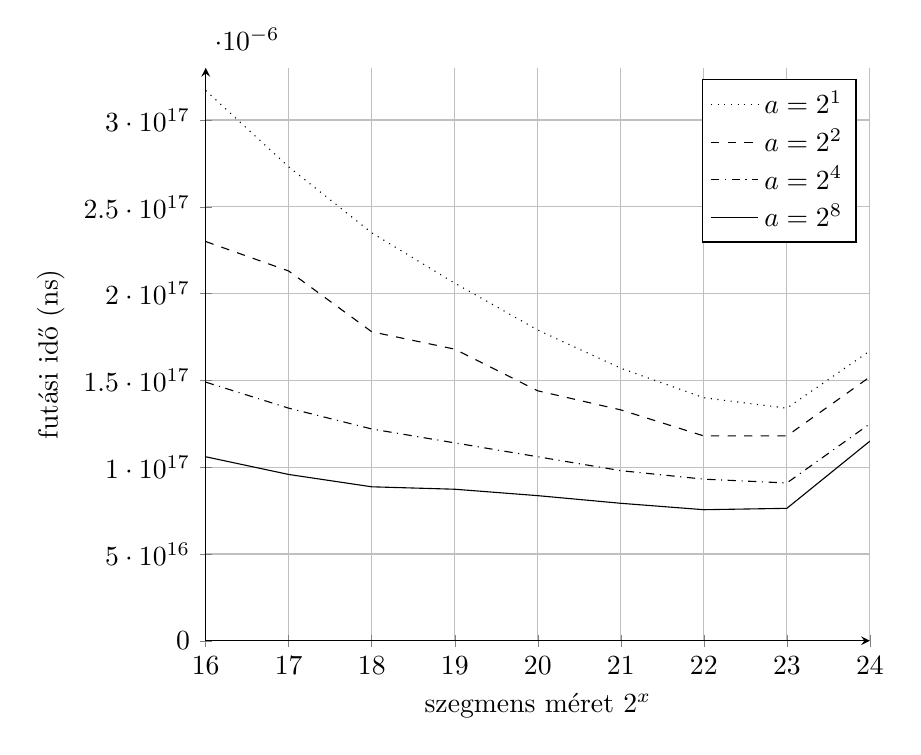
\begin{tikzpicture}

\begin{axis}[%
scale only axis,
xmin=16, xmax=24,
xlabel={szegmens méret $2^x$},
xmajorgrids,
ymin=0, ymax=3.3e11,scaled y ticks={base 10:6},
ylabel={futási idő (ns)},
ymajorgrids,
axis lines=left,
title={ },
legend style={nodes=right}]
\addplot [
color=black,
dotted
] coordinates {(16,3.17e11) (17,2.73e11) (18,2.35e11) (19,2.06e11) (20,1.79e11) (21,1.57e11) (22,1.40e11) (23,1.34e11) (24,1.67e11)};
\addlegendentry{$a=2^1$};
\addplot [
color=black,
dashed
] coordinates {(16,2.30e11) (17,2.13e11) (18,1.78e11) (19,1.68e11) (20,1.44e11) (21,1.33e11) (22,1.18e11) (23,1.18e11) (24,1.52e11)};
\addlegendentry{$a=2^2$};
\addplot [
color=black,
dashdotted
] coordinates {(16,1.49e11) (17,1.34e11) (18,1.22e11) (19,1.14e11) (20,1.06e11) (21,9.80e10) (22,9.31e10) (23,9.09e10) (24,1.25e11)};
\addlegendentry{$a=2^4$};
\addplot [
color=black,
solid
] coordinates {(16,1.06e11) (17,9.58e10) (18,8.87e10) (19,8.73e10) (20,8.36e10) (21,7.92e10) (22,7.55e10) (23,7.63e10) (24,1.15e11)};
\addlegendentry{$a=2^8$};

\end{axis}
\end{tikzpicture}
\end{figure}

\pagebreak
\subsubsection{Az edénysor helyessége}

Egy szám számjegyenkénti felírásából, és $h$ definíciójából következik, hogy
\begin{equation}
\label{kisebb}
x_{h(x, y)} < y_{h(x, y)}\ (x, y \in \mathbb{N}_0, x<y)
\end{equation}

A sor pozíciójának pontosan eggyel növelésének következménye, hogy a legnagyobb megváltozott helyiértéken eggyel nő a számjegy, és az összes kisebb helyiértéken a legnagyobb számjegy 0-ra vált. Ha $x=p(q)$, $y=p(q)+1$, $d'=d(x, y)$, $k=h(x, y)$, akkor
\begin{equation}
\label{eggyel}
x_k+1=y_k
\end{equation}
\begin{equation}
\label{valtozatlan}
\forall i \in \mathbb{N}, i > k: x_k=y_k
\end{equation}
\begin{equation}
\label{szamjegy}
\forall i \in \mathbb{N} , i < k : x_k = a-1 \textrm{ és } y_k = 0
\end{equation}

A sor elejének eltávolítása algoritmus helyessége következik abból, hogy a $d'$-nél kisebb indexű edények üresek, a $d'$-nél nagyobb indexű edények elemeinek távolsága nem változik a sor pozíciójának növelésével, és a $d'$ edény elemeit az algoritmus újrarendezi.
\begin{equation}
\label{ures}
\forall i \in \mathbb{N}_0, i<d': b(q, i) = \emptyset
\end{equation}
\begin{equation}
\label{marad}
\forall i \in \mathbb{N}_0, i>d': \forall r \in b(q, i) : i = d(p(q), p(r)) = d(p(q)+1, p(r))
\end{equation}

\ref{ures} bizonyításához tegyük fel indirekt, hogy $\exists i < d': \exists r \in b(q, i)$.
Legyen $k'=h(p(q), p(r))$. Az indirekt feltevés szerint
\begin{align*}
d(p(q), p(r)) = i < d' = d(p(q), p(q)+1)
\end{align*}
Ha $k' \not = k$, akkor $k' < k$, de \ref{kisebb} és \ref{szamjegy} ellentmondáshoz vezet:
\begin{align*}
p(q)_{k'} = a-1 < p(r)_{k'} = 0
\end{align*}
Ha $k' = k$, akkor $i < d'$ és \ref{ddef} miatt $p(r)_k < (p(q)+1)_k$. Ekkor \ref{kisebb} és \ref{eggyel} ellentmond egymásnak:
\begin{align*}
p(q)_k < p(r)_k < (p(q)+1)_k = p(q)_k + 1
\end{align*}
Tehát az indirekt feltevés ellentmondáshoz vezet, azaz \ref{ures} igaz, a $d'$-nél kisebb indexű edények üresek.

Legyen $i \in \mathbb{N}_0, i>d', r \in b(q, i), k'=h(p(q), p(r))$.
Ha $k' = k$, akkor
\begin{align*}
d(p(q), p(r)) = (a-1)k'+p(r)_k-1=d(p(q)+1, p(r))
\end{align*}
Ha $k \not = k'$, akkor \ref{ddef} szerint $k < k'$.
\ref{valtozatlan} szerint
\begin{align*}
p(q)_{k'} &= (p(q)+1)_{k'} \\
h(p(q), p(r)) &= k' = h(p(q)+1, p(r)) \\
d(p(q), p(r)) &= (a-1)k'+p(r)_k-1=d(p(q)+1, p(r))
\end{align*}
Ezek alapján \ref{marad} igaz, az elem távolsága nem változik a sor elejéhez képest.

%%% Local Variables:
%%% mode: latex
%%% TeX-master: "szakdolgozat"
%%% End:
